\documentclass[../main.tex]{subfiles}
\chapter{Simulation}
\label{c:simulation}

\begin{figure}
	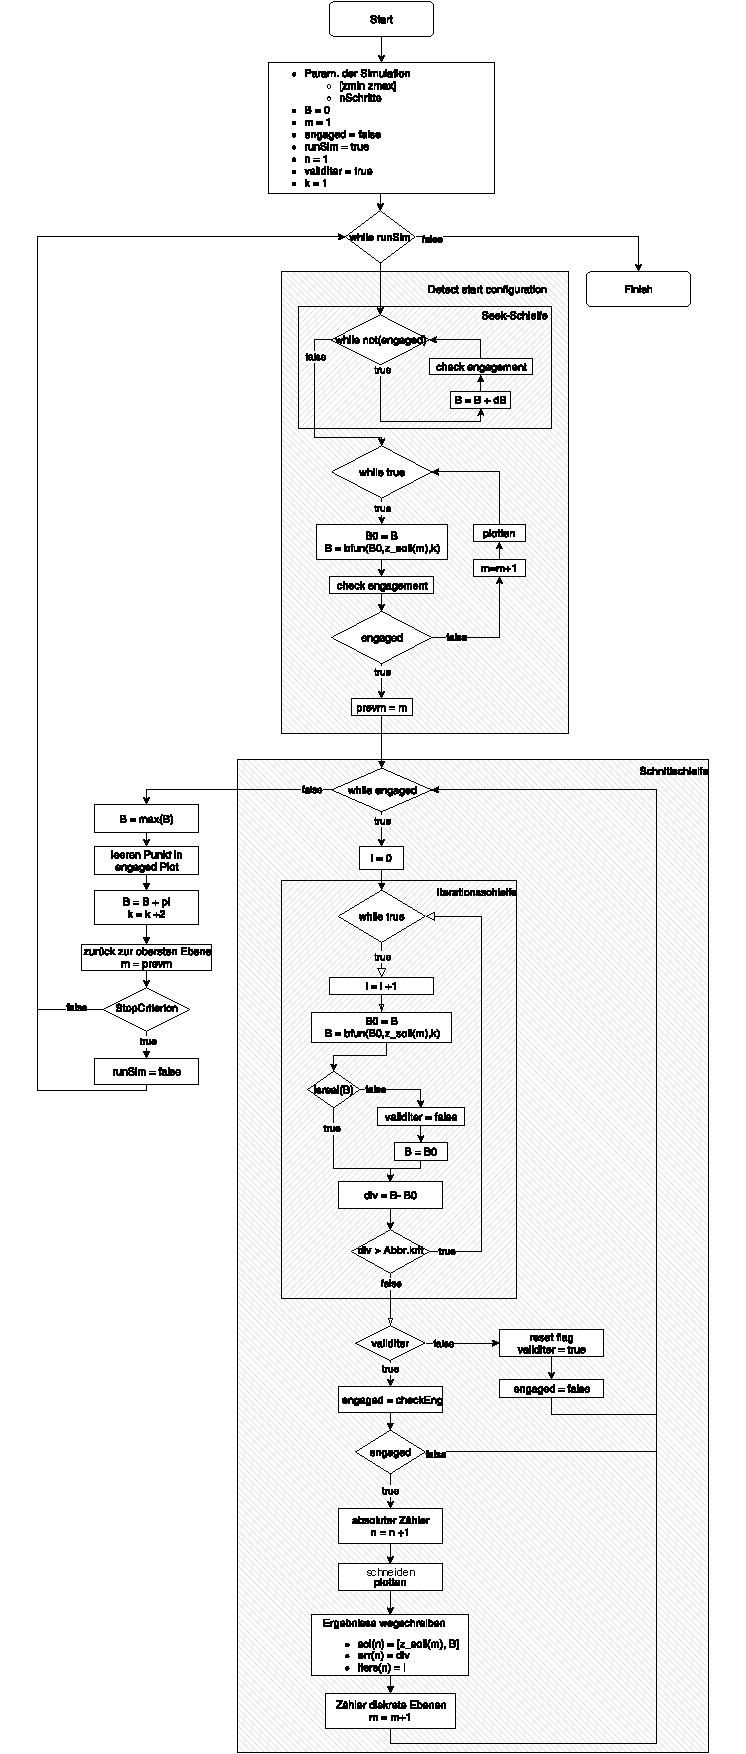
\includegraphics[scale=0.75]{vf1-flowchart}
	\caption{Hier ist die caption}
	\label{fig:flowchart}
\end{figure}

Abbildung \ref{fig:flowchart} zeigt das Flussbild der Simulation.
Der Ablauf der Simulation ist unterteilt in die Abschnitte Findung der Startkonfiguration, Durchführung der Schnitte mit den Lösungsiterationen, Erkennung des Schnittendes sowie Nachbereitung des Schnittes und schließlich Abschluss der Simulation.
Neben der Ausführung des Simulationscodes sollte der Status der Berechnung in Form von grafischen Ausgaben dargestellt werden.
Das Plotten von Daten in Echtzeit ist schwierig zu realisieren in \matlab, vor Allem bei dreidimensionalen Datensätzen.
Die standardmäßig zur Verfügung gestellten Routinen sind nicht gut optimiert für schnelle Ausführungszeit und es ist notorisch schwierig \matlab Code multithread-fähig zu gestalten.
Die Lösungsansätze um trotz dieser Herausforderungen die für die grafische Ausgabe beanspruchte Rechenzeit effizient zu nutzen und die Simulation möglichst geringfügig zu belasten wird ebenfalls besprochen.


Die einzelnen Prozessschritte der Simulation werden im Folgenden erläutert.

\section{Vorbereitung der Simulation}
Vor Beginn der Simulation wird die Simulationssteuerungsparameter eingelesen.
Dabei werden zunächst die Eingabedaten des betrachteten Falles festgelegt.
Mit folgende Parameter kann definiert werden, wie dieser Fall gestaltet ist:
\begin{itemize}
	\item Zähnezahl des Zahnrades
	\item Modul des Zahnrades
	\item Geometrie des des Werkzeuges (Durchmesser, Kopf- und Fußhöhe)	
\end{itemize}
Aus diesen Parametern können weitere Startbedingungen ermittelt werden.
So ist die Startposition des Werkzeugs und den daraus folgenden Positionen der Maschinenkomponenten zu berechnen wie sie in Abschnitt \ref{c:maschkomppos} besprochen wurden.
Die Position der X-Achse der Maschine wird berechnet über den Achsabstand des gedachten Schneckengetriebes nach \cite[Gleichung 23.4]{Matek2017}:
\begin{equation*}
	a = \frac{d_{s1}+d_{s2}}{2}
\end{equation*}
\begin{eqdscr}{$d_{s1}$, $d_{s2}$}
	\item[$a$] Achsabstand
	\item[$d_{s1}$, $d_{s2}$] Teilkreisdurchmesser von Schneckenrad und Schnecke
\end{eqdscr}
Der Teilkreisdurchmesser des Schneckenrades wird berechnet nach \cite{Matek2017}:
\begin{equation*}
	d_{s1} = m \cdot z
\end{equation*}
\begin{eqdscr}{$m$}
	\item[$m$] Modul
	\item[$z$] Zähnezahl des Werkstückes
\end{eqdscr}
Der Vorschubfaktor der X-Achse $\feed{X}{\wz}$ ist im betrachteten Fall 0, sie verändert also ihre Position ausgehend von der Startposition im Verlauf der Simulation nicht.

Für den Startwert der Y-Achse müssen die Größen $y$, Achsverschiebung im Ausgang, und $\yshift$ festgelegt werden.
Ebenso ist für den Achsvorschub der Y-Achse $\feed{Y}{\wz}$ ein Wert einzugeben.
Diese Größen sind im betrachteten Fall 0.
Die Y-Achse verändert im betrachteten Fall ihrer Position ausgehend von ihrem Startwert nicht.

Danach wird die Werkzeuggeometrie erzeugt.
Wie in Kapitel \ref{c:werkzeugkinematik} erläutert wird die Geometrie des Werkzeuges in Polarkoordinaten beschrieben.
Dabei wird im aktuellen Stand das Bezugsprofil durch vier Eckpunkte dargestellt, deren Koordinaten mit einem Algorithmus von \scherbarth berechnet werden.
Da eine Zahnstange als Zahnrad mit unendliche großer Zähnezahl verstanden werden kann, hat sie gerade Flanken \cite[Kap. 3]{Widmer1981}.
Eine Annäherung der Zahnstange mit vier Punkten ist deswegen zweckmäßig, obwohl Verrundungen am Zahnkopf damit noch nicht dargestellt werden können.

Die Simulation beginnt mit einem Ebenenindex m von 1.
Es wird davon ausgegangen, dass die erste ebene des Werkstücks geschnitten wird.
Vor jedem Schnitt wird dann die oberste Ebene ermittelt, die eine valide Schnittkonfiguration hervorbringt.
Wie diese Erkennung funktioniert wird in Abschnitt \ref{c:seeken} erläutert.

\section[Startkonfiguration]{Finden der Startkonfiguration}
\label{c:startkonfig}
Der erste Schritt zur Findung der Startkonfiguration bei jeder Werkzeugumdrehung ist die Suche nach der ersten validen Schnittkonfiguration.
Dieser Vorgang wird als Seeken, eine deutsche Form des englischen Wortes für ,,Suchen'', bezeichnet.

Eine valide Schnittkonfiguration tritt auf, wenn ein Punkt des Werkzeugs auf der Höhe einer diskreten Ebene des Werkstücks liegt.
Bei der vorliegenden Simulation ist das Werkstück entlang seiner Ausdehnung in z-Richtung in diskrete Ebenen unterteilt, welche das Werkzeug auf der jeweiligen Höhe in $z$ schneiden.
Die dabei entstehende Verschneidungsgeometrie des Werkstücks mit der Ebene ist eine zweidimensionale Geometrie.
Diese Geometrie ist ein Polygon, welches mit der Menge diskreter Punkte beschrieben, die seine Ecken darstellen.
Die Beschreibung von Werkstück und Werkzeug als Polygone wird in Abschnitt \ref{c:schnitte} im Detail beschrieben.

Seeken geschiet in der Seek-Schleife, die auch im Flussdiagrams in Abbildung \ref{fig:flowchart} beschrieben ist.
Dabei wird der Winkel des Werkzeugs ausgehend vom seiner Startkonfiguration mit einer bedatbaren Schrittweite inkrementiert, bis ein Punkte der Werkzeugschneide in der Hüllgeometrie des Werkstücks liegt.
Befindet sich ein Punkt des Werkzeugs in Hüllgeometrie des Werkstücks ist das Werkzeug ,,engaged'', von englisch ,,eingerastet''; die Schneide befindet sich im Eingriff.

Die Hüllgeomtrie des Werkstücks entspricht der Form des Rohmaterials, also ein Zylinder mit dem Durchmesser und der Höhe des Werkstücks.
Die Lage des Werkstücks entlang der z-Achse des Bearbeitungstischkoordinatensystems ist definierbar.
Die Berechnung des Engagements, also des Eingriffs der Schneide, muss sehr häufig erfolgen und deswegen sehr günstig sein, also wenig Rechenzeit in Anspruch nehmen.

Grundsätzlich muss ein Kompromiss zwischen der Größe der Schrittweite beim Seeken und der dafür notwendigen Rechenzeit gefunden werden.
Allerdings kann mit einem nachträglichen Schritt eine Überschreitung in den Werkstück-Envelope hinein geschickt ausgeglichen werden.

Engagement wird in der Funktion \code{checkEng} durch Berechnung der Schneideneckpunktkoordinaten in einem Zylinderkoordinatensystem erkannt.
Dieses Zylinderkoordinatensystem ist im Ursprung des Werkzeugkoordinatensystems aufgespannt ist.
Vergleichbar zu den überlagerten kartesischen und zylindrischen Koordinatensystemen des Werkzeugs, kann auch das Werkstück in kartesischen und zylindrischen Koordinatensystemen beschrieben werden.
Die Koordinaten eines Punktes werden dann durch einen Winkel, einen Radius und eine Höhe in z-Richtung beschrieben.

Damit ein Punkte als engaged gilt, müssen zwei Bedingungen erfüllt sein:
Zum einen muss der der Abstand eines Punktes zum Ursprung kleiner als der Radius des Werkstücks sein.
Zum anderen muss der Wert der z-Koordinate im Interval der Ausdehung des Werkstücks liegen.
Der Winkel des Punktes spielt zur Engagementerkennung keine Rolle.
Der Abstand $d$ des Punktes zum Urpsrung wird als euklidische Norm berechnet nach \cite{mwVecnorm}:
\begin{equation*}
	d = \|v\| = \sqrt{\sum_{k=1}^{N} \|v_k\|^2}
\end{equation*}
Die Funktion gibt dann als logischen Wert zurück, ob der Werkzeugpunkt engaged ist oder nicht.

Das Ziel des Findens der Startkonfiguration es, die Rotation des Werkzeuges zu finden, bei welcher das Werkzeug das Werstück gerade berührt.
Der Seek liefert einen Werkzeugwinkel, der in der Nähe dieser Konfiguration liegt.

Das Erkennen einer Engagementkonfiguration geschieht durch Vergleichen der Eckkoordinaten der Schneide
Nach Finden einer Werkzeugkonfiguration bei der mindes

\section{Durchführen der Schnitte}
\label{c:schnitte}
ist eine Position des Werkzeuges, bei der es durch Projektion der Schneide des Werkzeuges auf eine Werkstückebene zu einer Überlagerung kommt.
Werkzeug und Werkstück werden in der Simulation als Polygone repräsentiert, die in Matlab als Objekt der Klasse polyshape dargestellt werden.
Polyshape Objekte haben Methoden, die es erlauben Verschneidungsoperationen durchzuführen.
Dabei wird von einem polyshape Objekte die Geomtrie abgezogen, die von dem anderen Polygon überlagert wird.
\begin{figure}
	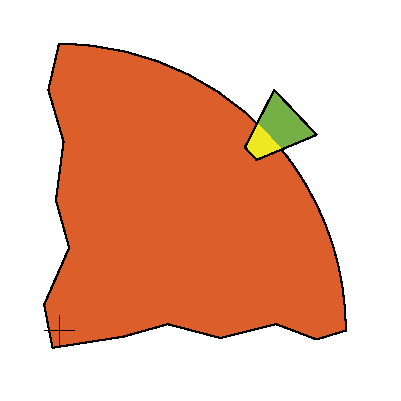
\includegraphics{uberlagerung}
	\caption{Hier ist die caption}
	\label{fig:uberlagerung}
\end{figure}
Bei einer Überlagerung


\section{Plotten}
Die Architektur des Codes erlaubt das parallel zum Lösen des mathematischen Problems die Ausgabe erfolgt mit minimalem Einfluss auf die Ausführungsgeschwindigkeit der Berechnung.
Das wurde erreicht durch die Auslagern des Plottens in eine Klasse.
